\chapter{Korrelation und Kausalität}
Eine der häufigsten Anwendungen der künstlichen Intelligenz ist die Vorhersage von Daten. Dabei wird ein Modell erstellt, das auf Basis von vorhandenen Daten Vorhersagen für zukünftige Daten trifft.

Bevor wir uns mit der Vorhersage von Daten befassen, sollten wir zuerst einige grundlegende Begriffe klären.

\cref{fig:Korrelationen} zeigt zwei Beispiele für Datenreihen (Variablen). Die linke Grafik zeigt eine Datenreihe der Verteilung der Noten sowie der Haarlänge in einer weiblichen Schulklasse. Die rechte Grafik zeigt eine Datenreihe der Nutzung von Social Media und der allgemeinen Lebenszufriedenheit der BenutzerInnen.

\begin{figure}[H]
	\centering
	\begin{subfigure}[t]{0.48\textwidth}
		\centering
		\includegraphics[width=\linewidth]{"Grundlagen_Info/10_KI_und_Algorithmen/Figures/haarlange_vs_notenschnitt"}
		\caption{Haarlänge und Notenschnitt in einer Schulklasse}
	\end{subfigure}
	~
	\begin{subfigure}[t]{0.48\textwidth}
		\centering
		\includegraphics[width=\linewidth]{"Grundlagen_Info/10_KI_und_Algorithmen/Figures/socialmedia_vs_zufriedenheit"}
		\caption{Social-Media-Nutzung und Zufriedenheit}
	\end{subfigure}
	\caption{Beispiele für Korrelationen}
	\label{fig:Korrelationen}
\end{figure}

Die linke Grafik zeigt einen positiven Zusammenhang zwischen der Haarlänge und der Schulnote. Bei der Interpretation solcher Daten ist Vorsicht geboten: Es könnte sein, dass die Daten rein zufällig so aussehen. Wenn man mehrere Klassen anschaut, sähe man eventuell keinen Trend. Eine allfällige These, wie etwa, dass längere Haare zu besseren Noten führen, müsste in einem wissenschaftlichen Experiment überprüft werden. Tiefere Analysen sind notwendig, um den Zusammenhang zwischen den Variablen zu verstehen.

Die rechte Grafik zeigt einen negativen Zusammenhang zwischen der Nutzung von Social Media und der Zufriedenheit. Wenn die Nutzung von Social Media steigt, sinkt die Zufriedenheit. Auch hier ist Vorsicht geboten: Es könnte sein, dass Menschen, die unzufrieden sind, mehr Zeit in sozialen Medien verbringen. Es könnte aber auch sein, dass die Nutzung von Social Media selbst unglücklicher macht. Auch hier ist eine tiefere Analyse notwendig, um den Zusammenhang zwischen den Variablen zu verstehen.

In beiden Fällen kann lediglich ein Zusammenhang zwischen zwei Variablen beobachtet werden. In der linken Grafik erkennt man: \enquote{steigt A, steigt auch B}, bzw. \enquote{steigt B, steigt auch A} (linke Abbildung). In der rechten Grafik kann beobachtet werden: \enquote{steigt A, sinkt B}, bzw. \enquote{steigt B, sinkt  A}. In diesen Fällen spricht man von einer \textbf{Korrelation}. Eine Korrelation beschreibt eine statistische Beziehung zwischen zwei Variablen. Eine Korrelation bedeutet nicht zwangsläufig, dass eine Variable die andere beeinflusst. Es kann auch sein, dass beide Variablen von einer dritten Variable beeinflusst werden oder dass die Korrelation rein zufällig ist.
\begin{itemize}
	\item \textbf{Positive Korrelation} bedeutet, dass wenn eine Variable steigt, auch die andere Variable steigt.
	\item \textbf{Negative Korrelation} bedeutet, dass wenn eine Variable steigt, die andere Variable sinkt.
	\item \textbf{Keine Korrelation} bedeutet, dass es keinen linearen Zusammenhang zwischen den beiden Variablen gibt.
\end{itemize}

In diesem Kapitel werden wir uns mit den Begriffen Korrelation und Kausalität beschäftigen.

\section{Kausalität}

\begin{mydefinition}[Kausalität]\label{def:kausalitaet}
\textbf{Kausalität} beschreibt eine Ursache-Wirkung-Beziehung zwischen zwei Variablen, welche wir im Allgemeinen A und B nennen.

Wenn eine Variable A (Ursache) eine andere Variable B (Wirkung) beeinflusst, spricht man in diesem Fall von Kausalität. Um zu beurteilen, ob eine Kausalität vorliegt, ist es wichtig, den Zusammenhang zwischen den Variablen zu analysieren und zu verstehen. Kausalität kann häufig nur durch wissenschaftliche  Experimente oder statistische Analysen nachgewiesen werden. Kausalität ist ein sehr komplexes Thema und es gibt viele verschiedene Arten von Kausalität.

Der Begriff \textit{Kausalität} hat seinen Ursprung im Lateinischen. Das Wort entstammt dem lateinischen Begriff \textit{causa}, was so viel wie Ursache bedeutet.

In der Regel wird Kausalität in fünf verschiedene Kategorien unterteilt:
\begin{enumerate}
	\item \textbf{Koinzidenz} (\enquote{nicht-Kausalität}) beschreibt eine zufällige Korrelation zwischen zwei Variablen, die keine kausale Beziehung haben. Die Variablen $A$ und $B$ treten zwar gemeinsam auf, doch $A$ und $B$ sind ohne Zusammenhang. Das gemeinsame Auftreten ist rein zufällig.
	      \begin{center}
		      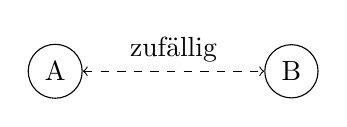
\begin{tikzpicture}
			      \node[circle, draw] (A) at (0,0) {A};
			      \node[circle, draw] (B) at (3,0) {B};
			      \draw[<->, dashed] (A) -- (B) node[midway, above] {zufällig};
		      \end{tikzpicture}
	      \end{center}
	      Beispiel: \enquote{Der Konsum von Mozzarella-Käse sowie die verliehenen Bauingenieurs-Doktortitel in den USA sind zwischen den Jahren 2000 bis 2009 beide angestiegen.}
	\item \textbf{Zyklische Beeinflussung} beschreibt eine Situation, in der zwei Variablen sich gegenseitig beeinflussen (gegenseitige Verstärkung im positiven oder negativen Sinn).
	      \begin{center}
		      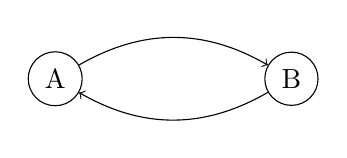
\begin{tikzpicture}
			      \node[circle, draw] (A) at (0,0) {A};
			      \node[circle, draw] (B) at (3,0) {B};
			      \draw[->] (A) to[bend left] (B);
			      \draw[->] (B) to[bend left] (A);
		      \end{tikzpicture}
	      \end{center}
	      Beispiel: \enquote{Schlafmangel führt zu mehr Stress, was wiederum zu mehr Schlafmangel führt.}
	\item \textbf{Gemeinsamer Grund} beschreibt eine Situation, in der eine dritte Variable C sowohl A als auch B beeinflusst.
	      \begin{center}
		      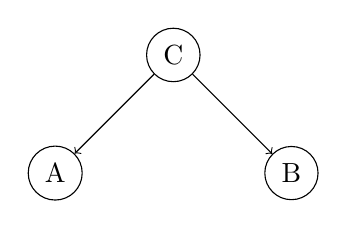
\begin{tikzpicture}
			      \node[circle, draw] (C) at (1.5,1.5) {C};
			      \node[circle, draw] (A) at (0,0) {A};
			      \node[circle, draw] (B) at (3,0) {B};
			      \draw[->] (C) -- (A);
			      \draw[->] (C) -- (B);
		      \end{tikzpicture}
	      \end{center}
	      Beispiel: \enquote{Zwischen November und Januar steigen sowohl der Verkauf von Winterreifen als auch die Häufigkeit von Erkältungen an (Grund: Jahreszeit).}

	\item \textbf{Indirekte Kausalität} beschreibt eine Situation, in der Variable A Variable B beeinflusst, aber nicht direkt, sondern via eine dritte Variable C.
	      \begin{center}
		      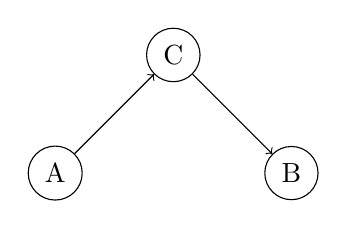
\begin{tikzpicture}
			      \node[circle, draw] (A) at (0,0) {A};
			      \node[circle, draw] (C) at (1.5,1.5) {C};
			      \node[circle, draw] (B) at (3,0) {B};
			      \draw[->] (A) -- (C);
			      \draw[->] (C) -- (B);
		      \end{tikzpicture}
	      \end{center}
	      Beispiel: \enquote{Sport führt zu besserem Schlaf, was wiederum zu besseren Prüfungsergebnissen führt.}
	\item \textbf{Direkte Kausalität} beschreibt eine Situation, in der Variable A Variable B direkt beeinflusst.
	      \begin{center}
		      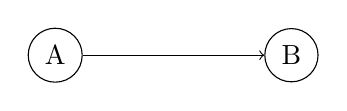
\begin{tikzpicture}
			      \node[circle, draw] (A) at (0,0) {A};
			      \node[circle, draw] (B) at (3,0) {B};
			      \draw[->] (A) -- (B);
		      \end{tikzpicture}
	      \end{center}
	      Beispiel: \enquote{Mehr Video-Streams führen automatisch zu mehr Einnahmen für die Youtuberin.}
\end{enumerate}
\end{mydefinition}

\begin{myexercise}
	In einer Klasse wurde ein Programmier-Test durchgeführt. Die SchülerInnen mussten 10 Fragen beantworten. Für jede richtige Antwort gab es 1 Punkt, für jede falsche Antwort gab es 0 Punkte. Die SchülerInnen wurden anschliessend in eine Rangliste eingeteilt, wobei die Person mit den meisten Punkten den ersten Platz belegte. Tabelle \ref{tab:rangliste} zeigt die Ergebnisse des Tests. Vervollständigen Sie die fehlenden Daten. Um welche Art von Zusammenhang (siehe \cref{def:kausalitaet}) handelt es sich?
	\begin{table}[H]
		\centering
		\begin{tabular}{clrr}
			\midrule
			Nr. & Name         & Anzahl Punkte & Rang \\
			\midrule
			1   & Anna Keller  & 2.5           & 5    \\
			2   & Jonas Meier  & 4.0           & ?    \\
			3   & Lara Schmid  & 1.0           & 7    \\
			4   & Elias Huber  & 3.5           & 3    \\
			5   & Mia Müller   & 5.0           & 1    \\
			6   & Noah Fischer & 2.0           & ?    \\
			7   & Sofia Weber  & 3.0           & 4    \\
			\midrule
		\end{tabular}
		\caption{Rangliste des Programmier-Tests}
		\label{tab:rangliste}
	\end{table}
	\begin{myanswer}
		Der Rang lässt sich direkt aus der Anzahl Punkte ableiten: Jonas belegt den 2. Rang und Noah den 6. Rang. Es handelt sich um eine \textbf{direkte Kausalität}, da die Rangliste direkt von der Anzahl Punkte abhängt. Wenn jemand mehr Punkte hat, hat er / sie auch einen höheren Rang.
	\end{myanswer}
\end{myexercise}

\begin{myexercise}
	Bestimmen Sie für folgende Aussagen, welche Art von Kausalität vorliegt:

	\begin{enumerate}
		\item Die Durchschnittsnote in der Klasse steigt über das Schuljahr hinweg. Im gleichen Zeitraum haben die Lehrpersonen ihren Kaffeekonsum gesteigert.
		\item In den Sommermonaten nehmen sowohl die Anzahl Sonnenbrände als auch der Verkauf von Glacé zu.
		\item In den letzten zehn Jahren hat der Konsum von Avocados in der Schweiz zugenommen. Im selben Jahrzehnt ist die Zahl bestandener Maturaprüfungen gestiegen.
		\item Eine Studie hat gezeigt, dass HunderbesitzerInnen weniger Risiko haben, übergewichtig zu werden.
		\item Eine Untersuchung von 1000 SchülerInnnen hat gezeigt, dass SchülerInnen, welche sehr gestresst sind, schlechtere Noten erzielen.
	\end{enumerate}

	\begin{myanswer}
		\begin{itemize}
			\item \textbf{Koinzidenz}: Keine kausale Beeinflussung. Die Korrelation ist zufällig, oder höchstens durch eine Drittvariable erklärbar (z.B. die Lehrpersonen investieren mehr Zeit in den Unterricht $\rightarrow$ mehr Stress $\rightarrow$ mehr Kaffee).
			      \begin{center}
				      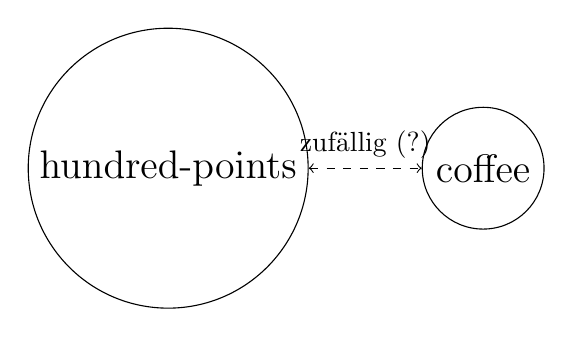
\begin{tikzpicture}
					      \node[circle, draw] (A) at (0,0) {\Large\emoji{hundred-points}};
					      \node[circle, draw] (B) at (4,0) {\Large\emoji{coffee}};
					      \draw[<->, dashed] (A) -- (B) node[midway, above] {zufällig (?)};
				      \end{tikzpicture}
			      \end{center}

			\item \textbf{Gemeinsamer Grund}: Beide Grössen werden durch eine gemeinsame Drittvariable beeinflusst: das Wetter bzw. die Jahreszeit.
			      \begin{center}
				      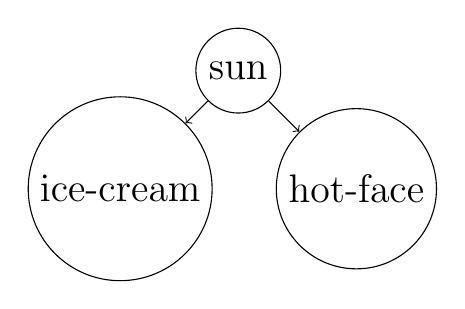
\begin{tikzpicture}
					      \node[circle, draw, minimum size=1cm] (C) at (1.5,1.5) {\Large\emoji{sun}};
					      \node[circle, draw, minimum size=1cm] (A) at (0,0) {\Large\emoji{ice-cream}};
					      \node[circle, draw, minimum size=1cm] (B) at (3,0) {\Large\emoji{hot-face}};
					      \draw[->] (C) -- (A);
					      \draw[->] (C) -- (B);
				      \end{tikzpicture}
			      \end{center}

			\item \textbf{Koinzidenz}: Keine echte Beeinflussung. Es handelt sich um eine Scheinkorrelation ohne sinnvollen Zusammenhang. Der gleichzeitige Trend ist rein zufällig, es sei denn, die Forschung zeige auf, dass Avocados eine positive Wirkung auf die kognitiven Fähigkeiten haben.
			      \begin{center}
				      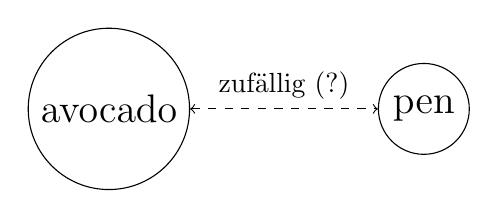
\begin{tikzpicture}
					      \node[circle, draw] (A) at (0,0) {\Large\emoji{avocado}};
					      \node[circle, draw] (B) at (4,0) {\Large\emoji{pen}};
					      \draw[<->, dashed] (A) -- (B) node[midway, above] {zufällig (?)};
				      \end{tikzpicture}
			      \end{center}

			\item \textbf{Indirekte Kausalität}: HundebesitzerInnen bewegen sich mehr, was zu weniger Übergewicht führt. Es handelt sich um eine indirekte Kausalität.
			      \begin{center}
				      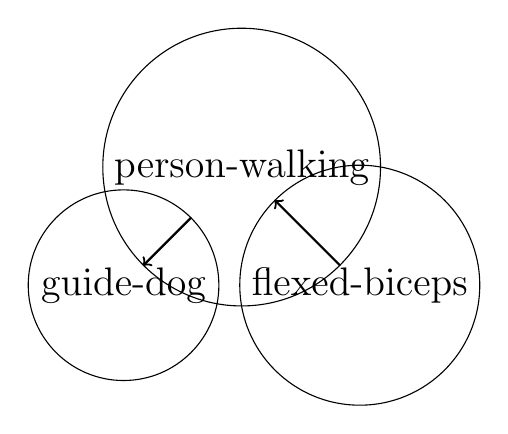
\begin{tikzpicture}
					      \node[circle, draw, minimum size=1cm] (A) at (0,0) {\Large\emoji{guide-dog}};
					      \node[circle, draw, minimum size=1cm] (C) at (1.5,1.5) {\Large\emoji{person-walking}};
					      \node[circle, draw, minimum size=1cm] (B) at (3,0) {\Large\emoji{flexed-biceps}};
					      \draw[->, thick] (A) -- (C);
					      \draw[->, thick] (C) -- (B);
				      \end{tikzpicture}
			      \end{center}

			\item \textbf{Zyklische Beeinflussung}: Stress führt zu schlechteren Noten, was wiederum zu mehr Stress führt. Es handelt sich um eine zyklische Beeinflussung.
			      \begin{center}
				      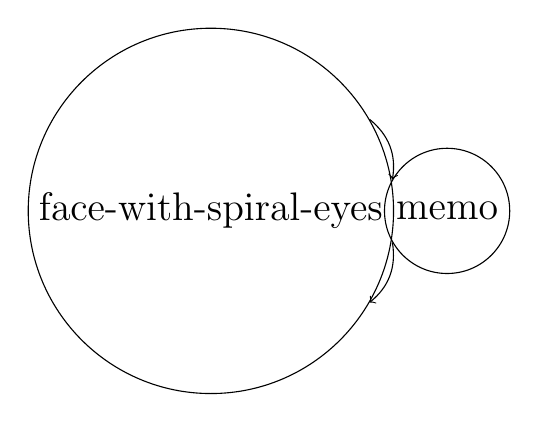
\begin{tikzpicture}
					      \node[circle, draw] (A) at (0,0) {\Large\emoji{face-with-spiral-eyes}};
					      \node[circle, draw] (B) at (3,0) {\Large\emoji{memo}};
					      \draw[->] (A) to[bend left] (B);
					      \draw[->] (B) to[bend left] (A);
				      \end{tikzpicture}
			      \end{center}
		\end{itemize}
	\end{myanswer}
\end{myexercise}

\section{Korrelation}

\begin{mydefinition}[Korrelation]

\textbf{Korrelation} beschreibt eine Beziehung zwischen zwei Variablen. Das Wort Korrelation kommt von den lateinischen Wörtern \textit{co(n)-} $=$ \enquote{mit} und \textit{relatio} $=$ Beziehung, was soviel wie eine gegenseitige Beziehung oder auch Wechselbeziehung bedeutet (\emoji{arrows-counterclockwise}). Im Kern bedeutet dies lediglich eine statistische Beziehung zwischen zwei Variablen (Beobachtungen) $A$ und $B$.

Eine Korrelation bedeutet nicht zwangsläufig, dass eine Variable die andere beeinflusst (siehe \cref{def:kausalitaet}). Es kann auch sein, dass beide Variablen von einer dritten Variable beeinflusst werden oder dass die Korrelation rein zufällig ist.
\begin{itemize}
	\item \textbf{Positive Korrelation} bedeutet, dass wenn eine Variable steigt, auch die andere Variable steigt.
	\item \textbf{Negative Korrelation} bedeutet, dass wenn eine Variable steigt, die andere Variable sinkt.
	\item \textbf{Keine Korrelation} bedeutet, dass es keinen linearen Zusammenhang zwischen den beiden Variablen gibt.
\end{itemize}

Der Korrelationskoeffizient wird typischerweise als Zahl $r$ angegeben, welche sich zwischen -1 (perfekte negative Korrelation) und 1 (perfekte positive Korrelation) bewegt. Ein Wert von 0 bedeutet, dass es keinen linearen Zusammenhang zwischen den beiden Variablen gibt (siehe \cref{fig:korr-r-bsp}). Dies schliesst jedoch nicht aus, dass es einen anderen, nicht-linearen Zusammenhang gibt.

\begin{figure}[H]
	\centering
	\foreach \corr in {-1, -0.8, -0.4, 0, 0.4, 0.8, 1} {\begin{subfigure}[t]{0.16\pagewidth}
				\centering
				\includegraphics[width=\linewidth]{"Grundlagen_Info/10_KI_und_Algorithmen/Figures/correlation_\corr"}
				\caption{r=\textbf{\corr}}
			\end{subfigure}
		}
	\begin{subfigure}[t]{0.16\pagewidth}
		\centering
		\includegraphics[width=\linewidth]{"Grundlagen_Info/10_KI_und_Algorithmen/Figures/correl_ex_15"}
		\caption{r$\simeq$\textbf{0}}
	\end{subfigure}
	\caption{Beispiele für den Korrelationskoeffizienten $r$}
	\label{fig:korr-r-bsp}
\end{figure}

\end{mydefinition}

\cref{fig:Korrelationen} zeigt zwei Beispiele für Korrelationen. In der linken Grafik ist eine positive Korrelation zwischen der Haarlänge und dem Notendurchschnitt zu sehen. In der rechten Grafik ist eine negative Korrelation zwischen der Nutzung von Social Media und der Zufriedenheit zu sehen.

Um Zusammenhänge zwischen zwei Variablen nicht nur zu benennen, sondern auch quantifizieren und vergleichen zu können, wäre es hilfreich, den Zusammenhang zwischen zwei Datenreihen in einer einzigen Zahl $r$ ausdrücken zu können. Hilfreich wäre es zudem, falls diese Zahl positiv wäre bei positiven Korrelationen und negativ bei negativer Korrelation. Damit könnten Fragen wie die Folgende beantwortet werden:

\enquote{Welcher Zusammenhang ist stärker --- Schlafdauer vs. Konzentration ($r = 0.6$) oder Handynutzung vs. Noten ($r = --0.4$)?}

In Psychologie, Wirtschaft, Medizin oder Sport begegnet man Korrelationen oft: z.B. \enquote{Bewegung korreliert mit geringerer Krankheitsanfälligkeit}. Wer $r$ versteht, kann solche Aussagen kritisch beurteilen und Studienergebnisse kritisch interpretieren.

Die Stärke der Korrelation zwischen zwei Variablen kann durch eine mathematische Formel berechnet werden. Eine Möglichkeit, dies zu tun, ist die Berechnung des Korrelationskoeffizienten \(r\).

Der erste Schritt zur Berechnung des Korrelationskoeffizienten ist die Berechnung der Mittelwerte aller Variablen, $\overline{x}$ und $\overline{y}$ (siehe erste Abbildung in \cref{fig:Korrelationen-Abweichung}). Der Mittelwert ist der arithmetische Durchschnittswert aller Werte einer Variablen.

In einem zweiten Schritt berechnen wir die Abweichung der ursprünglichen Werte von ihrem Mittelwert (siehe zweite Grafik in \cref{fig:Korrelationen-Abweichung}).  Die Abweichung eines Wertes \(x_i\) von seinem Mittelwert \(\overline{x}\) wird als \( x_i' \) bezeichnet.

\begin{figure}[H]
	\centering
	\begin{subfigure}[t]{0.48\textwidth}
		\centering
		\includegraphics[width=\linewidth]{"Grundlagen_Info/10_KI_und_Algorithmen/Figures/polizei_vs_kriminalitaet_correl"}
		\caption{Ursprüngliche Daten}
	\end{subfigure}
	~
	\begin{subfigure}[t]{0.48\textwidth}
		\centering
		\includegraphics[width=\linewidth]{"Grundlagen_Info/10_KI_und_Algorithmen/Figures/polizei_vs_kriminalitaet_correl_norm"}
		\caption{Daten als Abweichung vom Mittelwert}
	\end{subfigure}
	\caption{Korrelations-Beispiel mit Abweichung vom Mittelwert}
	\label{fig:Korrelationen-Abweichung}
\end{figure}

Wie man in \cref{fig:Korrelationen-Abweichung} erkennen kann, sieht die Abbildung der Daten als Abweichung vom Mittelwert fast gleich wie die ursprünglichen Werte selber aus, ausser dass die Werte jetzt um 0 zentriert sind. Somit kann man folgenden \enquote{Trick} anwenden, um den Korrelationskoeffizienten zu berechnen: Wir multiplizieren die Abweichungen der beiden Variablen miteinander und addieren die Produkte auf. Das Ergebnis ist eine Zahl, die den Zusammenhang zwischen den beiden Variablen beschreibt. Wenn die Daten im roten oder blauen Bereich liegen, ist das Produkt \(x_i' \cdot y_i'\) positiv. Wenn die Daten im grünen oder gelben Bereich liegen, ist das Produkt negativ.

Wir berechnen nun also die Zahl \(Z\):

\[
	Z = x_1' \cdot y_1' + x_2' \cdot y_2' + \dots + x_n' \cdot y_n'
\]


\begin{myexercise}\label{ex:z-excel}
	Verwenden Sie die Excel-Datei auf Moodle und berechnen Sie die Zahl \(Z\) für die beiden Datenserien. Welche Korrelation liegt vor? Ist es eine positive oder negative Korrelation?
	\begin{myanswer}
		\begin{itemize}
			\item Die Korrelation zwischen der Berufserfahrung (Jahre) und der Einladungswahrscheinlichkeit beträgt \(Z = 44.66\). Es handelt sich um eine positive Korrelation.
			\item Die Korrelation zwischen der Nutzung von Social Media und der Zufriedenheit beträgt \(Z = -30.13\). Es handelt sich um eine negative Korrelation.
		\end{itemize}
	\end{myanswer}
\end{myexercise}
\begin{myexercise}\label{ex:z-excel2}
	Verwandeln Sie in Aufgabe \cref{ex:z-excel} die Anzahl Jahre Berufserfahrung in eine neue Variable, die die Anzahl Jahre Berufserfahrung in Monaten angibt. Berechnen Sie die Zahl \(Z\) für die beiden Datenserien. Wie verändert sich die Korrelation?
	\begin{myanswer}
		Die Korrelation zwischen der Berufserfahrung (Monate) und der Einladungswahrscheinlichkeit beträgt nun neu \(Z = 18.78\). Der Korrelationswert hat sich also nur aufgrund einer andere Grösseneinheit verändert. Dies wirft die Frage auf, wie man einen Korrelationskoeffizienten erschaffen könnte, der nicht von der Grösseneinheit abhängt.
	\end{myanswer}
\end{myexercise}

Wie wir in \cref{ex:z-excel2} gesehen haben, ist die Zahl \(Z\) von der Grösseneinheit abhängig. Das bedeutet, dass wir die Stärke der Korrelation nicht direkt vergleichen können, wenn die Variablen unterschiedliche Grösseneinheiten haben. Um dies zu lösen, verwenden wir den \textbf{Korrelationskoeffizienten \(r\)}, welcher die Zahl \(Z\) zwischen -1 und 1 normiert:
\begin{equation}
	\begin{aligned}
		r & = \frac{Z}{\sqrt{\lr{(x_1')^2 + (x_2')^2 + \dots + (x_n')^2} \cdot \lr{(y_1')^2 + (y_2')^2 + \dots + (y_n')^2}}} \\
		  & = \frac{Z}{\sqrt{\lr{\displaystyle\sum_{i=1}^n (x_i')^2} \cdot \lr{\displaystyle\sum_{i=1}^n (y_i')^2}}}
	\end{aligned}
\end{equation}


Der Korrelationskoeffizient \(r\) ist eine standardisierte Version der Zahl \(Z\). Der Korrelationskoeffizient \(r\) liegt immer zwischen -1 und 1. Ein Wert von 1 bedeutet, dass die beiden Variablen in einem perfekten positiven linearen Zusammenhang stehen. Ein Wert von -1 bedeutet, dass die beiden Variablen in einem perfekten negativen linearen Zusammenhang stehen. Ein Wert von 0 bedeutet, dass es keinen linearen Zusammenhang zwischen den beiden Variablen gibt. Dies schliesst jedoch nicht aus, dass es einen anderen, nicht-linearen Zusammenhang gibt.

\begin{myexercise}
	Berechnen Sie den Korrelationskoeffizienten \(r\) für die beiden Datenserien in \cref{ex:z-excel}. Wie stark ist die jeweilige Korrelation?
	\begin{myanswer}
		\begin{itemize}
			\item Die Korrelation zwischen der Berufserfahrung (Jahre) und der Einladungswahrscheinlichkeit beträgt \(r = 0.96\). Es handelt sich um eine sehr starke positive Korrelation.
			\item Die Korrelation zwischen der Nutzung von Social Media und der Zufriedenheit beträgt \(r = -0.83\). Es handelt sich um eine starke negative Korrelation.
		\end{itemize}
	\end{myanswer}
\end{myexercise}

\begin{myexercise}
	Ordnen Sie die folgenden Bilder steigend nach dem Korrelationskoeffizienten \(r\) ein. Welches Bild hat den höchsten Korrelationskoeffizienten? Welches Bild hat den tiefsten Korrelationskoeffizienten?
	\begin{figure}[H]
		\centering
		\foreach \i in {7,12,3,18,5,10,1,15,8,14,2,17,6,11,4,16,9,13} {
				\begin{subfigure}[t]{0.22\textwidth}
					\centering
					\includegraphics[width=\linewidth]{"Grundlagen_Info/10_KI_und_Algorithmen/Figures/correl_ex_\i.pdf"}
					\caption{$r = \_\_\_$}
				\end{subfigure}
			}
	\end{figure}
\end{myexercise}

\begin{myexercise}
	Luca und Mira bereiten sich auf eine Prüfung vor. Sie erfassen während der Vorbereitung drei Grössen:
	\begin{itemize}
		\item \textbf{B:} \textbf{B}eginn der Lernphase (z.\,B. 8.5 = 8:30 Uhr)
		\item \textbf{D:} \textbf{D}auer der Lerneinheit in Stunden
		\item \textbf{A:} \textbf{A}nzahl bearbeiteter Seiten pro Tag
	\end{itemize}
	Die folgende Tabelle zeigt die Korrelationen zwischen diesen drei Variablen:

	\begin{table}[H]
		\centering
		\begin{tabular}{l||c|c|c}

			              & \textbf{B und D} & \textbf{B und A} & \textbf{D und A} \\
			\midrule\midrule
			\textbf{Luca} & $-0.69$          & $-0.04$          & $0.25$           \\\midrule
			\textbf{Mira} & $0.64$           & $0.54$           & $0.89$           \\
		\end{tabular}
	\end{table}

	\begin{enumerate}
		\item Beantworten Sie folgenden Fragen mit \enquote{Luca}, \enquote{Mira}, \enquote{beide}, oder \enquote{keine}.:
		      \begin{enumerate}
			      \item Wer lernt länger, wenn er oder sie ausgeschlafen ist? \hfill \textit{(B kleiner = früherer Start)}
			      \item Bei wem hat der Zeitpunkt des Lernstarts keinen Einfluss auf die Anzahl bearbeiteter Seiten?
			      \item Bei wem führt eine längere Dauer der Lerneinheit zu einer höheren Anzahl bearbeiteter Seiten?
		      \end{enumerate}
		\item \textbf{Wer braucht insgesamt weniger Zeit, um den gesamten Stoff durchzuarbeiten?}
	\end{enumerate}

	\begin{myanswer}
		\begin{enumerate}
			\item Erste Fragen
			      \begin{enumerate}
				      \item Bei B und D gibt es bei \textbf{Mira} eine positive Korrelation: Wenn sie länger schläft (später aufsteht), lernt sie länger.
				      \item Bei B und A gibt es bei \textbf{Luca} eine Korrelation von fast 0: Der Zeitpunkt des Lernstarts hat keinen Einfluss auf die Anzahl bearbeiteter Seiten.
				      \item Bei \textbf{beiden} gibt es eine positive Korrelation: Wenn die Dauer der Lerneinheit steigt, steigt auch die Anzahl bearbeiteter Seiten. Bei Mira ist die Korrelation jedoch viel stärker (0.89) als bei Luca (0.25).
			      \end{enumerate}
			\item Das kann aufgrund der gegebenen Information nicht mit Sicherheit gesagt werden. Man bräuchte dazu genauere Kenntnisse über die Daten.
		\end{enumerate}
	\end{myanswer}
\end{myexercise}